\mychapter{Potències i arrels}{Potències i arrels}{
\includegraphics[width=4cm]{img-02/radicales}}{chap:potencies}

 \vsoo
 \begin{iniaval}
 \textbf{Completa:}


\begin{itemize}
\item En una potència $b^n$, $b$ es diu \dotfill i $n$ s'anomena \dotfill

\item  Per multiplicar potències d'igual base, copiam la base i \dotfill els exponents.

\item  Per dividir potències d'igual base, copiam la base i \dotfill els exponents.

\item  Per elevar una potència a una potència, copiam la base i \dotfill els exponents.

\end{itemize}
\vspace{0.5cm}
 \textbf{Sense emprar la calculadora, calcula el valor de:}

\begin{tasks}(3)
\task ${\left(-2\right)}^3=$   \task  ${\left(-2\right)}^4=$   \task  $5^0=$ 

\task  $\sqrt{144}=$   \task $4^{-1}$ =   \task $\sqrt[3]{8}=$
 \end{tasks}

\vspace{0.5cm}
 \textbf{Expressa com una única potència:}
\begin{tasks}[resume=true](3)
\task $ 5^8\textrm{·}5^3\textrm{·}5\ =$ \task ${(-3)}^5:{(-3)}^2=$     \task ${\left(7^3\right)}^5\ =$
\end{tasks}
\vspace{0.5cm}
\end{iniaval}
\addanswersline{Avaluació inicial}{0}{base;\par exponent;\par sumam;\par restam; \par multiplicam.\par \begin{tasks}(2)
		\task --8 \task 16 \task 1 \task 12 \task $\frac{1}{4}$ \task 2 \task $5^{12}$ \task $(-3)^3$ \task $7^{15}$
\end{tasks}	
}


\newpage
\section{Potències}

\begin{center}
	\renewcommand*\baselinestretch {1.25}
	
	\begin{theorybox}
		
		\begin{minipage}{0.75\textwidth}
			\video[ytid=s7moTUkU6w8]{121}{Potències. Definició i propietats}
			
			
			\textbf{\textit{Valor numèric de potències}}
			
			\textbf{Potència d'exponent natural: }
			
			Recorda que $b^{0} = 1$ \, i \, $b^{1} = b$
			
			$(-3)^{2}= (-3)\cdot(-3)=+9$  \quad   mentre que 
			
			$(-3)^{3} = (-3)\cdot(-3)\cdot(-3)=-27$
			
			En general, el signes de les potencies és:
			
		\end{minipage}
		\begin{minipage}{0.25\textwidth}
			\centering
			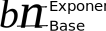
\includegraphics[width=0.7\textwidth]{img-02/potencia}
		\end{minipage}
		
		\begin{longtable}{|p{1.4in}|p{1.3in}|p{1.3in}|} \hline 
			\rowcolor{lightgray}\textbf{$b^{n}$} & \textit{$n$ parell} & \textit{$n$ imparell} \\ \hline 
			\cellcolor{lightgray}\textit{$b$ positiu} & \textbf{+} & \textbf{+} \\ \hline 
			\cellcolor{lightgray}\textit{$b$ negatiu} & \textbf{+} & \textbf{--} \\ \hline 
		\end{longtable}
		
	\end{theorybox}
\end{center}

\begin{mylist}

\exer \mental Determina el signe de les potències:  a) ($-$1)${}^{9}$ \quad b) ${(-5)}^{12}$  \quad c) ($-$12)${}^{5}$ \quad   d) (--8)${}^{4}$ 
\answers{[Negatiu, Positiu, Negatiu, Positiu]}

\exer  \spen Calcula el valor numèric de les potències
\begin{tasks}(2)
 \task ${\left(-3\right)}^4=$ 
 
 \task ${\left(-2\right)}^3=$ 
 
 \task ${\left(-1\right)}^{415}=$ 
 
 \task $\ {\left(-4\right)}^1=$
 
 \end{tasks}
\answers[cols=2]{[$81$, $-8$, $-1$, $-4$]}
  
\end{mylist}

\begin{example}
 \textbf{Potència de base racional: }Com calculam la potència quan la base és una fracció?

    S'eleva el numerador i el denominador a l'exponent ${\left(\frac{3}{5}\right)}^2=\frac{3^2}{5^2}=\ \frac{9}{25}$
\end{example}


\begin{mylist}
\exer \spen Calcula el valor numèric de les potències
\begin{tasks}(2)
\task  ${\left(\frac{3}{2}\right)}^4=$   \task ${\left(\frac{1}{5}\right)}^3=$  \task ${\left(-\frac{9}{4}\right)}^0=$  \task $\ {\left(\frac{-3}{4}\right)}^3=$
 \end{tasks}
\end{mylist}
\answers[cols=2]{[$\dfrac{81}{16}$, $\dfrac{1}{125}$, $1$, $-\dfrac{27}{64}$]}

\begin{theorybox}
 \textbf{Elevar un nombre a $-1$}: Significa calcular la inversa del nombre, per exemple
\[{\mathrm{3}}^{\mathrm{-}\mathrm{1}}\mathrm{=}\frac{\mathrm{1}}{\mathrm{3}};   \quad\quad\quad\quad  {\left(\frac{\mathrm{3}}{\mathrm{5}}\right)}^{\mathrm{-}\mathrm{1}}\mathrm{=}\frac{\mathrm{5}}{\mathrm{3}}\] 
\end{theorybox}

\begin{mylist}

\exer \spen Calcula el valor numèric de les potències
\begin{tasks}(2)
\task  ${\left(-3\right)}^{-1}=$   \task $2^{-1}=$   \task ${\left(-\frac{1}{4}\right)}^{-1}=$   \task $\ {\left(\frac{4}{7}\right)}^{-1}=$
\end{tasks}
\answers[cols=2]{[$-\dfrac{1}{3}$, $\dfrac{1}{2}$, $-4$, $\dfrac{7}{4}$]}
\end{mylist}


\begin{theorybox}

 \textbf{Potència d'exponent negatiu: }Què significa elevar a un exponent negatiu?

 Primer elevam a $-1$ que significa fer la inversa de la base, després elevam a l'exponent positiu:
\[{\mathrm{3}}^{\mathrm{-}\mathrm{2}}\mathrm{=}\frac{\mathrm{1}}{{\mathrm{3}}^{\mathrm{2}}}=\frac{1}{9}     ; \quad\quad\quad\quad {\left(\frac{\mathrm{3}}{\mathrm{5}}\right)}^{\mathrm{-}\mathrm{2}}\mathrm{=}{\left(\frac{\mathrm{5}}{\mathrm{3}}\right)}^{\mathrm{2}}=\frac{5^2}{3^2}=\frac{25}{9}\] 

\end{theorybox}

\begin{mylist}
\exer \spen Calcula el valor numèric de les potències
\begin{tasks}(2)
 \task ${\left(-3\right)}^{-3}=$  \task $2^{-4}=$   \task ${\left(-\frac{1}{4}\right)}^{-2}=$  \task$\ {\left(\frac{4}{7}\right)}^{-3}=$
\task $\left(\frac{5}{4}\right)^{3}$ =  \task $-\left(\frac{2}{7}\right)^{-4}$ =  
\task $\left(-\frac{1}{6}\right)^{4}$ = \task $\left(-\frac{5}{2}\right)^{-2}$ =
 \end{tasks}
\end{mylist}
\answers{[$-\dfrac{1}{27}$, $\dfrac{1}{16}$, $16$, 
	$\dfrac{343}{64}$, $\dfrac{125}{64}$, $-\dfrac{2041}{16}$, $1296$, $\dfrac{4}{25}$]}


\begin{theorybox}[Propietats de les potències]
\begin{minipage}[t]{0.82\textwidth}
	 \begin{tabular}{p{0.4\textwidth}p{0.6\textwidth}}
\textbf{Producte d'igual base:}  & ${\mathrm{b}}^{\mathrm{n}}\mathrm{\textrm{·}}{\mathrm{b}}^{\mathrm{m}}\mathrm{=\ }{\mathrm{b}}^{\mathrm{n+m}}$ \\ [0.25cm]

\textbf{Quocient d'igual base:}  & ${\mathrm{b}}^{\mathrm{n}}\mathrm{:}{\mathrm{b}}^{\mathrm{m}}\mathrm{=}\frac{{\mathrm{b}}^{\mathrm{n}}}{{\mathrm{b}}^{\mathrm{m}}}\mathrm{=\ }{\mathrm{b}}^{\mathrm{n-m}}$
\\[0.25cm]
\textbf{Potència de potencia:    } & ${{\mathrm{(b}}^{\mathrm{n}}\mathrm{)}}^{\mathrm{m}}\mathrm{=\ }{\mathrm{b}}^{\mathrm{n\textrm{·}m}}$
\\[0.25cm]
\textbf{Operacions d'igual exponent:} & ${\mathrm{a}}^{\mathrm{n}}\mathrm{\textrm{·}}{\mathrm{b}}^{\mathrm{n}}\mathrm{=\ }{\left(\mathrm{a\textrm{·}b}\right)}^{\mathrm{n}}$ \quad\quad ${\mathrm{a}}^{\mathrm{n}}\mathrm{:}{\mathrm{b}}^{\mathrm{n}}\mathrm{=\ }{\left(\mathrm{a:b}\right)}^{\mathrm{n}}$
\end{tabular}
\end{minipage}
\fbox{
\begin{minipage}{0.13\textwidth}
	\centering
	\textbf{Recorda:}
	\par
		
		$b^0=1$
		
		$b^1= b$
	
\end{minipage}
}
\end{theorybox}

\begin{mylist}
\exer \spen Expressa en forma d'una única potència:  

\begin{tasks}(2)
\task   ($-$7)${}^{3}$ · ($-$7)${}^{5}$ · ($-$7)${}^{2}$ · ($-$7)${}^{6 }$=    \task   3${}^{2}$ · 3${}^{7}$ · 3 · 3${}^{4}$ · 3${}^{3}$${}^{ }$=

 \task   ($-$6)${}^{4}$ · ${4}^{4}$ · ($-$1)${}^{4}$ · ($-$5)${}^{4}$=   \task  ($-$8)${}^{9}$: ($-$8)${}^{3}$  =

\task   ($-$3)${}^{2}$ :  ($-$3)${}^{7}$ =    \task   (+75)${}^{4}$ : ($-$3)${}^{4}$  =  

 \task  ($-$5)${}^{8}$ : ${8}^{8}$=    \task   (($-$2)${}^{5}$)${}^{6}$${}^{ }$=
\answers{[$(-7)^{16}$, $3^{17}$, $120^4$, $8^6$, $(-3)^{-3}$, $(-25)^4$, $(-5/8)^8$, $(-2)^{30}$]}


 \end{tasks}


\exer  Expressa com a única potència d'exponent positiu:  

\begin{tasks}(2)
\task  (\textbf{$-$}3/4)${}^{3}$ · (\textbf{$-$}3/4)${}^{2}$ · (\textbf{$-$}3/4)\textbf{${}^{-}$}${}^{8}$ =  \task   (1/8)\textbf{${}^{-}$}${}^{5}$· (1/8)${}^{4}$·(1/8)${}^{-}$${}^{2}$${}^{ }$=
\task   (5/4)${}^{6}$ · (\textbf{$-$}2/3)${}^{6}$· (\textbf{$-$}1/7)${}^{6}$ =  \task   (\textbf{$-$}3/5)${}^{-}$${}^{4}$ · (\textbf{$-$}3/8)${}^{-}$${}^{4}$ · (\textbf{$-$}1/4)\textbf{${}^{-}$}${}^{4}$${}^{ }$=
 \task   ($-$2/5)${}^{4}$ : ($-$2/5)${}^{7}$ =   \task    (5/8)${}^{3}$ : (5/8)${}^{-}$${}^{2}$${}^{ }$=
 \task    (1/5)${}^{-}$${}^{3}$ : (2/9)${}^{-}$${}^{3}$ =    \task    ($-$6)${}^{5}$ : (-2/9)${}^{5}$${}^{ }$=
\end{tasks}
 \answers{[$\left(-\frac{4}{3} \right)^{2}$, $\left(\frac{1}{8} \right)^{-3}=8^3$, $\left(\frac{5}{42} \right)^6$, $\left(\frac{160}{9} \right)^4$, $\left(-\frac{5}{2} \right)^3$, $\left(\frac{5}{8} \right)^5$, $\left(\frac{10}{9} \right)^3$, $27^5$]}


\exer Expressa en forma d'única potència:
\begin{tasks}(2)
\task 2${}^{5 }$ · ( -3)${}^{5}$ · ($-$1)${}^{5 }=$    \task ($-$1)${}^{3}$ · ($-$1)${}^{8}$ · ${(-1)}^{5}=$ 
\task  4${}^{3}$ · ($-$2)${}^{3}$· ($-$1)${}^{3 }$· 5${}^{3}=$    \task ($-$5)${}^{2}$ · ($-$5)${}^{4}=$  
\task ($-$9)${}^{2}$ · 9${}^{3}$ · 9${}^{4}$ · 9=     \task ($-$18)${}^{4}$: ($-$3)${}^{4}=$   
\task ${6}^{5} : {6}^{2}=$     \task ($-$3)${}^{2}$: ($-$3)${}^{4}=$
\end{tasks}
\answers{[$6^5$, $1$, $40^3$, $5^6$, $9^{10}$, $6^4$, $6^3$, $(-3)^{-2}$]} 


\exer  Expressa en forma de potència d'exponent positiu:  
\begin{tasks}(2)
 \task ($-$4) ${}^{-}$${}^{3 }$     \task ${9}^{-}$${}^{3}$  \task ($-$2)${}^{5}$: ($-$2)${}^{9}$  \task $(-5) \cdot (-5)^{2} : (-5)^{6}$
\end{tasks}
\answers[cols=2]{[$\left(\frac{-1}{4}\right)^3$, $\left(\frac{1}{9}\right)^3$, $\left(\frac{1}{2}\right)^4$, $\left(\frac{-1}{5}\right)^3$]}

\exer  Expressa en forma d'única potència:
\begin{tasks}(2)
\task  $\left( \frac23 \right)^{3 } \cdot \left( \frac{-1}{5} \right)^{3} \cdot \left( \frac{-4}{9} \right)^{3} \cdot \left( \frac{1}{2} \right)^{3}$    

\task  
$\left( \frac{-1}{4} \right)^3\cdot \left( \frac{-1}{4} \right)^{-2}\cdot \left( \frac{-1}{4} \right)\cdot \left( \frac{-1}{4} \right)^4$

\task $\left( \left( \frac{-1}{3} \right)^4 \right)^{3/2} \cdot \left( \frac{2}{5} \right)^{6}$

\task  $\left( \frac{2}{5} \right)^{1/2}\cdot \left( \frac{2}{5} \right)^{3/4}\cdot \left( \frac{2}{5} \right)^{-1/6}$
%\task (7/8)${}^{3}$${}^{ }$: (1/6)${}^{3}$
\end{tasks}
\answers[cols=2]{[$\left(\frac{4}{135}\right)^3$, $\left(-\frac{1}{4}\right)^6$, $\left(\frac{-2}{15}\right)^6$, $\left(\frac{2}{5}\right)^{12/12}=\frac{2}{5}$]}
\end{mylist}



\section{Notació científica}

	
\begin{theorybox}
	\video[ytid=9JUpIa4ncWg]{158}{Potències de 10. Un zoom còsmic.}
	
	Un número escrit en notació científica és de la forma:
	\[ m \times \ 10^{e} \]
	on l'exponent $e$ s'elegeix perquè el nombre $m$, en valor absolut, sigui major o igual a 1 i menor que 10.
	
	Algunes potències de 10 importants
\begin{center}
	\renewcommand{\arraystretch}{1.2}
\begin{tabular}{|l|c|c|l|l|}
	\hline
	\rowcolor{lightgray} Distància (m) & Ordre & Símbol & Exemple \\
	\hline
	1000000000000 & $10^{12}$ & tera (T) & Distància de Saturn al Sol\\
	\hline
	1000000000 & $10^9$ & giga (G) & Radi del Sol \\
	\hline
	1000000 & $10^6$ & mega (M) & Radi de la Lluna \\
	\hline
	1000 & $10^3$ & kilo (k) & 1 km \\
	\hline
	1 & $10^0$ &  & 1 m \\
	\hline
	0,001 & $10^{-3}$ & mil·li (m) & Gruix d'un cabell \\
	\hline
	0,000001 & $10^{-6}$ & micro ($\mu$) & Cèl·lula \\
	\hline
	0,000000001 & $10^{-9}$ & nano (n) & Mol·lècula \\
	\hline
		0,000000000001 & $10^{-12}$ & pico (p) & Àtom \\
	\hline
\end{tabular} 
\end{center}
\end{theorybox}
 

\begin{blueshaded}
	
	\begin{minipage}{0.7\textwidth}
		\textbf{Notació científica amb la calculadora:}
		
		Per trobar el valor decimal d'una arrel necessitaràs una calculadora científica, com ara la de la figura. Tot seguit et mostram alguns exemples
		
		\begin{tabular}{lrl}
			$1,25\cdot 10^3$:  & \tecla{\quad$1.25$\quad}  \tecla{\quad EXP\quad}  \tecla{\quad$3$\quad}   \tecla{\quad=\quad} & \pantalla{1250} \\ [0.25cm] 
			$2,4\cdot 10^{-2}$:  & \tecla{\quad$2.4$\quad}  \tecla{\quad EXP\quad}  \tecla{\quad$-2$\quad}   \tecla{\quad=\quad} & \pantalla{0.024} \\ [0.25cm] 
		\end{tabular}
	  
	  \vspace{0.25cm}
	  La tecla \tecla{ENG} permet passar de notació normal a científica i viceversa, per exemple:
	  
	  	\begin{tabular}{lrl}
	  	$1250000$:  & \tecla{\quad$1250000$\quad}  \tecla{\quad=\quad}  \tecla{\quad ENG\quad}   & \pantalla{$1.25\times 10^{6}$} \\ [0.25cm] 
	  	$2,5\cdot 10^{-3}$:  & \tecla{\quad$2.5$\quad}  \tecla{\quad EXP \quad}  \tecla{\quad -3 \quad}   \tecla{\quad = \quad} & \\
	  	& \tecla{\quad SHIFT \quad}  \tecla{\quad ENG \quad}     & \pantalla{$0.0025\times 10^{0}$} \\ [0.25cm] 
	  \end{tabular}
		
	\end{minipage}
	\begin{minipage}{0.3\textwidth}
		\centering
		\includegraphics[width=0.9\textwidth]{img-02/fx82ms-a}
	\end{minipage}
	
	
	
\end{blueshaded}

\begin{mylist}

\exer \spen Expressa en notació científica:
\begin{tasks}(2)
\task 140000000 =    \task  32800 =  
\task  71000000000000000 =    \task  0,0000075 =
\task  $-$18000000 =     \task  0,00000000042 =
\task  $-$0,009 =    \task  0,00000000007 =
\end{tasks}
 \answers{[$\cient{1.4}{8}$, $\cient{3.28}{4}$, $\cient{7.1}{16}$, $\cient{7.5}{-6}$, $\cient{-1.8}{7}$, $\cient{4.2}{-10}$, $\cient{-9}{-3}$, $\cient{7}{-11}$]}

\exer  \simbolsearch Cerca informació expressada en notació científica sobre:
\begin{tasks}(2)
\task  La distància entre la Terra i la Lluna  \task  Unitat de massa atòmica
\task  Km que corresponen a un any llum  \task  Un gúgol   
\end{tasks}
\answers[cols=2]{[$\cient{3.84}{8}$ m, $\cient{1.66}{-27}$ kg, $\cient{9.46}{12}$ km, $\cient{10}{100}$]}


\exer[1]  Realitza les operacions i expressa el resultat en notació científica:
\begin{tasks}(2)
\task 4 · 10${}^{3}$ + 2,4 · 10${}^{6}$ -- 1,7 · 10${}^{5}$ -- 3 · 10${}^{3}$ \task 2,3 · 10${}^{-}$${}^{5}$ -- 3,45 · 10${}^{-}$${}^{4}$ + 6 · 10${}^{-}$${}^{3}$
\task  3 · 10${}^{-}$${}^{4}$ · 4,5 · 10${}^{2 }$   \task  1,8 · 10${}^{5}$: 5 · 10${}^{8}$
\end{tasks}
\answers[cols=2]{[$2.231\cdot 10^6$, $5.678\cdot 10^{-3}$, $1.35\cdot 10^{-5}$, $3.6\cdot 10^{-4}$]}


\exer[1]  L'estel Sirius està a uns 8,611 anys llum del nostre planeta. Expressa en metres, mitjançant notació científica la distància que recorreria una nau espacial que realitzés un trajecte d'anada i tornada a Sirius. (\textit{Recorda}: Un any llum, la longitud que recorre la llum en un any, és aproximadament igual a  9,46~$\times$~10${}^{12}$~km (9~460~730~472~580,8~km amb més aproximació))
\answers{$1.629\cdot 10^{17}$ m}

 

\vspace{-2cm}
\exer[1]  \begin{minipage}[t]{0.7\textwidth}  La massa d'un electró en repòs s'estima en 9,11 · 10${}^{-31}$ kg, la d'un protó és d'1,672 $\cdot$ 10${}^{-}$${}^{27}$ kg, i la d'un neutró 1,64 x 10${}^{-}$${}^{27}$ kg. Calcula la massa d'un àtom de carboni 14 (C${}_{14}$) format per sis protons, sis electrons i 6 + 2 = 8 neutrons. (El C${}_{14}$ és un isòtop que té dos neutrons més que el carboni normal i que s'utilitza per datar).
\end{minipage}
\begin{minipage}{0.3\textwidth}
\centering
\vspace{2cm}
\includegraphics[width=0.6\textwidth]{img-02/carbono14}
\end{minipage}
\answers{La massa de l'isòtop C${}_{14}$ és: $6\times 1,672 \cdot 10^{-27} + 6 \times 9,11 \cdot 10^{-31}+ 8\times 1,64 \cdot 10^{-27}  = 2.32\cdot 10^{-26}$ kg}

 
\vspace{3cm}

\exer  Calcula i expressa en notació científica:
\begin{tasks}(2)
 \task 0,00829 + 4 · 10${}^{-}$${}^{3}$ + 7,45 · 10${}^{-}$${}^{5}$      \task 5 · 10${}^{6}$ -- 2,8 · 10${}^{7}$ -- 3 · 10${}^{5}$
 \task 5 · 10${}^{-}$${}^{2}$ -- 4 · 10${}^{2}$ + 1,4 · 10${}^{-}$${}^{3}$     \task 3 · 10${}^{-}$${}^{5 }$ · (-- 2,7) · 10${}^{-}$${}^{3}$ + 4,2 · 10${}^{-}$${}^{6}$
\end{tasks}
\answers[cols=2]{[$\cient{1.236}{-2}$, $\cient{-2.33}{7}$, $\cient{-3.99}{2}$, $\cient{4.12}{-6}$]}
 


\exer[1]  S'estima que existeixen 40 milions de bacteris en un gram de terra. Expressa en notació científica de forma aproximada el nombre de bacteris que existeixen en uns camions que estan descarregant 50 tones mètriques d'arena en una platja.
\answers{$50 t \cdot \frac{1\,000\,0000 \text{ g}}{1 t} \cdot \frac{40\cdot 10^6 \text{ bacteris}}{1 \text{ g}}=4\cdot 10^{13}$ bacteris}

 


\exer  Si  \textit{x} = 240000; \textit{y =} 0,00058; \textit{z }= 7,2 · 10${}^{6}$: Calcula i expressa en notació científica 
\begin{tasks}(3)
 \task \textit{x·y}      \task 2\textit{x }+ \textit{y}·10${}^{7}$      \task 3\textit{x} -- 5\textit{y}
\end{tasks}
\answers{[$\cient{1.392}{2}$, $\cient{4.86}{5}$, $\cient{7.2}{5}$]}


\exer[1]  Arquimedes, en el seu tractat \textit{El arenario} explica una manera per expressar nombres molt grans, com el nombre de grans d'arena que hi ha en tota la Terra. Anem a estimar-los ara per un altre procediment. Estimem quants grans d'arena necessitem per tenir un gram. Suposa que 50 grans d'arena. S'estima que la massa de la Terra és de:  $M_T$=5 980 000 000 000 000 000 000 000 000 g = 598 \textbf{$\boldsymbol{\cdot}$} 10${}^{25}$ g

 Calcula de forma aproximada el nombre de grans d'arena que hi ha en tota la Terra.
 
\answers{$ 598 \cdot 10^{25} \text{ g} \cdot \frac{50 \text{ grans}}{1 \text{ g}} \approx 3\cdot 10^{29}$ grans d'arena}


 

\vspace{-2cm}
\exer  \begin{minipage}[t]{0.7\textwidth}
	\simbolsearch Cerca a Wikipèdia les masses i els radis dels planetes Júpiter i la Terra
	 % que la massa de Júpiter és d'1,898·10${}^{27}$ kg, i que la massa de la Terra és de 5,972·10${}^{24}$ kg.
	\begin{tasks}
	\task Calcula la relació de massa entre Júpiter i la Terra.
	%
	\task Quants de planetes Terra necessitam per ocupar el mateix volum que el planeta Júpiter? $V=\ofrac{4}{3}\pi R^3$
	%
	\task Calcula la relació de densitat ($d=M/V$) entre Júpiter i la Terra.
	\end{tasks}
	\answers{$M_J=1,898$·$10^{27}$ kg, $M_T=5,972$·$10^{24}$ kg, $R_J=69911$ km, $R_T=6371$ km, \par a) $\dfrac{M_J}{M_T} = 318$,\par b) $\dfrac{V_J}{V_T} = 1321$,   $\dfrac{d_J}{d_T} = 0.24$\par és un planeta gasós (de fet és menys dens que l'aigua).}
	
\end{minipage}
\begin{minipage}{0.3\textwidth}
	\centering
	\vspace{2cm}
	\includegraphics[width=0.6\textwidth]{img-02/jupiter}
\end{minipage}





\exer  Utilitza la calculadora per obtenir la teva edat expressada en segons en notació científica.
\answers{14 anys=$\cient{4.42}{8}$ s;\par 15 anys=$\cient{4.73}{8}$ s;\par 16 anys=$\cient{5.05}{8}$ s}

 


\exer  S'estima que el volum de l'aigua dels oceans és de 1~285~600~000 km${}^{3}$ i el volum d'aigua dolça és de 35~000~000 km${}^{3}$. Escriu aquestes quantitats en notació científica i calcula la proporció d'aigua dolça.
\answers{$\cient{1.2856}{9}$ km${}^{3}$ i $\cient{3.5}{7}$ km${}^{3}$.\par La proporció és 2.72 \%}

 


\exer  Se sap que en un àtom d'hidrogen el nucli constitueix el 99 \% de la massa, i que la massa d'un electró és aproximadament de  $9,109 \cdot 10^{-31}$ kg. Quina massa té el nucli d'un àtom d'hidrogen? (\textit{Recorda}: Un àtom d'hidrogen està format pel nucli, amb un protó, i per un únic electró).
\answers{Si tenim present que l'electró, que pesa 9,109 $\cdot$ 10${}^{-}$${}^{31}$ kg, representa únicament l'1 \%, només cal multiplicar per 100 i obtenim la massa de l'àtom: $\cient{9.109}{-29}$ kg}

 


\exer  A ne'n Joan li han fet una analítica de sang i té 5 milions de glòbuls vermells en cada mm${}^{3}$. Escriu en notació científica el nombre aproximat de glòbuls vermells que té en Joan estimant que té 5 litres de sang. (1 l=1 dm$^3$)
\answers{En Joan té $\cient{2.5}{9}$ glòbuls vermells}

\end{mylist}

\pagebreak
\section{Arrels o radicals}

\begin{theorybox}
	\begin{minipage}{0.35\textwidth}
		\centering
		\videonw[ytid=oIk7H9wenrM]{128}{Arrels: Definició}
	\end{minipage}
\begin{minipage}{0.35\textwidth}
	\centering
	\videonw[ytid=UTYWwJAcJfE]{130}{Radicals: Propietats}
\end{minipage}
\begin{minipage}{0.2\textwidth}
	\centering
	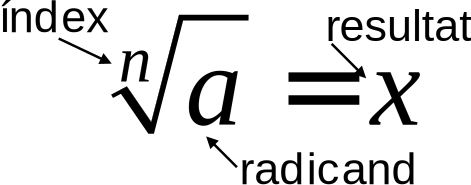
\includegraphics[width=0.9\textwidth]{img-02/radical}
\end{minipage}

\begin{center}
\begin{tabular}{llll}
Deim que l'arrel quadrada & $\sqrt{16}=4$ & perquè & $4^2 = 16$ \\
Deim que l'arrel cúbica  & $\sqrt[3]{125}=5$& perquè& $5^3 = 125$\\
Deim que l'arrel quarta  & $\sqrt[4]{16}=2$ &perquè& $2^4 = 16$\\
$\cdots$ & & & \\
En general l'arrel enèsima &$\sqrt[n]{a}=x$& perquè &$x^n = a$
\end{tabular}
\end{center}
\end{theorybox}

\begin{mylist} 


\exer  \spen  Escriu la llista dels 10 primers quadrats perfectes. 


\begin{longtable}{|p{0.5in}|p{0.3in}|p{0.3in}|p{0.3in}|p{0.3in}|p{0.3in}|p{0.3in}|p{0.3in}|p{0.3in}|p{0.3in}|p{0.3in}|} \hline 
\textbf{$n$} & 1 & 2 & 3 & 4 & 5 & 6 & 7 & 8 & 9 & 10 \\ \hline 
\textbf{$n^{2}$} &  &  &  &  &  &  &  &  &  &  \\ [0.5cm] \hline 
\end{longtable}
\answers{1, 4, 9, 16, 25, 36, 49, 64, 81, 100}

 
 \exer \mental  Calcula \textbf{mentalment} les següents arrels:
 \begin{tasks}(7)
 	\task  $\sqrt{49} $ \task  $\sqrt{25} $  \task  $\sqrt{100} $  \task  $\sqrt{64} $ \task $\sqrt{81} $  \task  $\sqrt{1} $   \task  $\sqrt{0} $
 \end{tasks}
\answers[cols=2]{[7, 5, 10, 8, 9, 1, 0]}
 
 \exer  \mental Calcula \textbf{mentalment} la part entera de les següents arrels:
 \begin{tasks}(7)
 	\task  $\sqrt{51} $ \task  $\sqrt{27} $  \task  $\sqrt{102} $  \task  $\sqrt{63} $ \task  $\sqrt{80} $  \task  $\sqrt{2} $            \task  $\sqrt{123} $
 \end{tasks}
 \answers[cols=2]{[7, 5, 10, 7, 8, 1, 11]}

 
 \end{mylist}

\vspace{0.5cm}

\begin{blueshaded}
	
	\begin{minipage}{0.7\textwidth}
		\textbf{Arrels amb la calculadora:}
		
		Per trobar el valor decimal d'una arrel necessitaràs una calculadora científica, com ara la de la figura. Tot seguit et mostram la combinació de tecles que has d'utilitzar.
		
		\begin{tabular}{lrl}
			$\sqrt[3]{5}$:  & \tecla{SHIFT}   \tecla{\quad$x^3$\quad}  \tecla{\quad5\quad}    \tecla{\quad=\quad} & \pantalla{1.709975947} \\ [0.25cm]
			$\sqrt[4]{3}$:  & \tecla{\quad4\quad}  \tecla{SHIFT}   \tecla{\quad$\wedge$\quad}  \tecla{\quad 3\quad}    \tecla{\quad=\quad} & \pantalla{1.316074013} 
		\end{tabular}
		
		\vspace{0.25cm}
		Les comprovacions de cada arrel són:
		
		
		\begin{tabular}{lrl}
			$1.709975947^3$:  & \tecla{1.709975947}   \tecla{\quad$\wedge$\quad}  \tecla{\quad3\quad}    \tecla{\quad=\quad} & \pantalla{5} \\ [0.25cm]
			$1.316074013^4$:  & \tecla{1.316074013}   \tecla{\quad$\wedge$\quad}  \tecla{\quad 4\quad}    \tecla{\quad=\quad} & \pantalla{3} 
		\end{tabular}
		
		
	\end{minipage}
	\begin{minipage}{0.3\textwidth}
		\centering
		\includegraphics[width=0.9\textwidth]{img-02/fx82ms-b}
	\end{minipage}
	
	
	
\end{blueshaded}


\begin{theorybox}

\begin{center}
	\begin{tabular}{l|c|c}
		 Signe de $\sqrt[n]{a}$ & $a>0$ & $a<0$ \\ \hline
		 $n$ parell & $+$ & No existeix \\ \hline
		 $n$ senar & $+$ & $-$
	\end{tabular}
\end{center}
\end{theorybox}


\begin{mylist}
  \exer \mental Indica quines arrels quadrades són nombres enters, quines nombres irracionals i quines no existeixen:
 \begin{tasks}(4)
 	\task  $\sqrt{36} $ \task  $\sqrt{-25} $  \task  $\sqrt{100} $ \task  $\sqrt{32} $ \task  $\sqrt[5]{-7} $  \task  $\sqrt{10} $            \task  $\sqrt{100}$ \task $\sqrt[3]{-125}$
 \end{tasks}
\answers{[entera, no, natural, irracional, irracional, irracional, entera, entera]}

 \exer  Calcula totes les solucions:  
 \begin{tasks}(5)
 	\task  $\sqrt{121} $   \task  $\sqrt[{3}]{-8} $  \task  $\sqrt[{4}]{10000} $  \task  $\sqrt[{5}]{-1} $      \task  $\sqrt[{7}]{1} $
 \end{tasks}
\answers{[$\pm 11$, --2, $\pm 10$, --1, 1]}
 
\end{mylist}

 \begin{theorybox}
  Tot radical o arrel es pot expressar com a potència d'exponent una fracció:
  $\sqrt[3]{5^2} = 5^{\ofrac{2}{3}}$
  
  i viceversa $2^{\ofrac{5}{4}}=\sqrt[4]{2^5}$. Fixeu-vos que l'índex de l'arrel és el denominador de l'exponent.
 \end{theorybox}
 
 \begin{mylist}
 	
 \exer \spen  Expressa en forma de radical:  
 \begin{tasks}(3)
 	\task  ($-$3)${}^{4/5}=$  \task  8${}^{1/3}=$   \task  5${}^{2/3}=$
 \end{tasks}
 \answers{[$\sqrt[5]{(-3)^4}$, $\sqrt[3]{8}$, $\sqrt[3]{5^2}$]}
 
 \exer \spen Expressa en forma d'arrel: 
 \begin{tasks}(4)
 	\task  ($-$4)${}^{3/5}=$  \task  7${}^{1/6   }=$ \task ${21}^{1/3 }=$  \task  ($-$5)${}^{2/3}=$
 \end{tasks}
\answers{[$\sqrt[5]{(-4)^3}$, $\sqrt[6]{7}$, $\sqrt[3]{21}$, $\sqrt[3]{(-5)^2}$]}
 
 \exer \spen  Expressa en forma de potència:  
 \begin{tasks}(4)
 	\task  $\sqrt[{5}]{6^{3} } $${}^{ }=$\task  $\sqrt{(-7)^{5} }=$ \task  $\sqrt{3^{5} }=$ \task  $\sqrt[{3}]{(-30)^{4} }=$
 \end{tasks}
\answers{[$6^{3/5}$, $(-7)^{5/2}$, $3^{5/2}$, $(-30)^{4/3}$]}
 
 \exer  Calcula: 
 \begin{tasks}(5)
 	\task  $\sqrt{12100} $  \task  $\sqrt{0,64}$   \task  $\sqrt[3]{-0,008}$  \task  $\sqrt[{5}]{-1} $  \task  $\sqrt{0,49} $
 \end{tasks}
\answers{[110, 0.8, --0.2, --1, 0.7]}
 
 \exer  Calcula: 
 \begin{tasks}(4)
 	\task  $\sqrt[{4}]{2,0736} $ \task  $\sqrt[{5}]{-0,00001} $${}^{ }$\task  $\sqrt{33640000} $  \task   $\sqrt[{3}]{-2,7\cdot 10^{-5} } $
 \end{tasks}

\answers{[1.2, --0.1, 5800, --0.03]}

\end{mylist}

\begin{theorybox}[Operacions amb radicals]
\textbf{Suma i resta:} Tan sols podem sumar i restar radicals idèntics
\[\boxed{2\sqrt{5} + 4 \sqrt{5}} - 7\sqrt{3}  = \boxed{ 6\sqrt{5} } - 7\sqrt{3}\]

\textbf{Producte i divisió de radicals d'igual índex:} 
\[ \sqrt{5}\cdot \sqrt{3} = \sqrt{15},  \quad\quad\quad \quad\quad\quad \frac{\sqrt{8}}{\sqrt{2}} = \sqrt{\frac{8}{2}}=\sqrt{4}=2 \]
\end{theorybox}

\vspace{2cm}
\begin{mylist}
 \exer  \spen Redueix:  
 \begin{tasks}(2)
 	\task  $3\sqrt{2} - 2\sqrt{2} + 7 \sqrt{2}=$  
 	
 	\task  $\frac{1}{2}\sqrt{5} + 3\sqrt{5} + \sqrt{5}=$  
 	
 	\task  $\sqrt{2} - 2\sqrt{3} + \frac{3}{4} \sqrt{2}=$
 	
 	\task  $-5\sqrt{7} + 3\sqrt{7} + 3 \sqrt{3}=$
 \end{tasks}
\answers[cols=2]{[$8\sqrt{2}$, $\frac{9}{2}\sqrt{5}$, $\frac{7}{4}\sqrt{2}-2\sqrt{3}$, $-2\sqrt{7}+3\sqrt{3}$]}

\end{mylist} 

\begin{theorybox}[Extreure factors d'un radical]
 En principi, les arrels $\sqrt{5} + \sqrt{20}$ no es poden ajuntar en una perquè són diferents. No obstant això, podem simplificar $\sqrt{20}$ extraient factors. 
 
 El primer que feim és \textbf{descomposar} el nombre en factors primers: $20 = 2^2 \cdot 5$
 
 \[ \sqrt{20} = \sqrt{ \boxed{2^2} \cdot 5} = \boxed{2} \sqrt{5} \]
 

``{  \normalfont \textit{tot el que està elevat a 2 dins una arrel quadrada surt defora de l'arrel sense l'exponent}}"
 
\end{theorybox}

\begin{resolt}[E]{
 Extreu factors 
 
  \[ \text{a) } \sqrt[3]{2 \cdot 5^3 } \]

 \[\text{b) } 5\sqrt{2^5 \cdot 3^2 } \]

 \[\text{c) } \sqrt[4]{162 } \]

 \[\text{d) } \sqrt[3]{32} \]
}

a) Tot el que està elevat a 3 surt de l'arrel cúbica $ \sqrt[3]{2 \cdot 5^3 }=  5 \sqrt[3]{2}$
\vspace{0.25cm}


b) Tot el que està elevat a 2 surt de l'arrel quadrada. Feim ``paquets'' si l'exponent supera a 2:  $  5\sqrt{2^5 \cdot 3^2 } = 5\sqrt{2^2 \cdot 2^2 \cdot 2 \cdot 3^2}=5\cdot 2 \cdot 2 \cdot 3\sqrt{ 2} =12 \sqrt{2}$
\vspace{0.25cm}


c) Descomposam el radicand i treim factors $ \sqrt[4]{162 }= \sqrt[4]{2\cdot 3^4 }= 3 \sqrt[4]{2}$
\vspace{0.25cm}

d) Descomposam el radicand, feim ``paquets'' i treim factors  $ \sqrt[3]{32}=\sqrt[3]{2^5}=\sqrt[3]{2^3 \cdot 2^2}=2\sqrt[3]{2^2}$ 
\end{resolt}

\begin{mylist}
 \exer[1]  Extreu els factors possibles en cada radical:  
 \begin{tasks}(3)
 	\task  $\sqrt[{4}]{a^{6\cdot } b^{5} } $  \task  $\sqrt[{3}]{6^{5} \cdot 3^{4} \cdot 2^{6} } $  \task  $\sqrt{4\cdot 5^{3} \cdot 9^{3} } $
 \end{tasks}
 \answers[cols=2]{[$a\cdot b\,\sqrt[4]{a^2 b}$, $6^2 \cdot 3 \cdot 2^2 \sqrt[3]{3\cdot 6^2}$, $90\,\sqrt{45}$]}
 
 \exer[1]  Extreu factors de cada radical: 
 \begin{tasks}(2)
 	\task  $\sqrt[{3}]{5^7} $   \task  $\sqrt{54} $    \task  $\sqrt{\frac{8}{9} } $        \task $\sqrt{\frac{x^{3} }{y^4} } $
 \end{tasks}
\answers[cols=2]{[$5^3\,\sqrt[{3}]{5}$, $3\sqrt{6}$, $\frac{2}{3}\sqrt{2}$, $\frac{x}{y^2}\sqrt{x }$]}
\end{mylist}

\pagebreak

 \begin{theorybox}[Arrel d'una arrel]
 	Una forma de calcular l'arrel d'una arrel és passar-les a forma de potència i operar les potències. Per exemple:
 	\[ \sqrt[3]{ \sqrt[4]{5} } = \left(5^\ofrac{1}{4}\right)^\ofrac{1}{3} =  \left(5 \right)^\ofrac{1}{12} = \sqrt[12]{5}  \]
 	
 	Una forma més còmoda i ràpida és simplement escriure una arrel d'índex el producte d'índexs:
 	
 	\[ \sqrt[n]{ \sqrt[m]{a} } =  \sqrt[n\cdot m ]{a}  \]
 	
 	
 	\includegraphics[width=0.75cm]{img-02/warning}  \textbf{Recorda que una arrel quadrada conté un índex 2:  $\sqrt{a}=\sqrt[ {\small 2}]{a}$}
 \end{theorybox}



\begin{mylist} 
 \exer  Expressa en forma d'única arrel:   
 \begin{tasks}(2)
 	\task  $\sqrt[{3}]{\sqrt{18} } $   \task  $\sqrt[{4}]{\sqrt[{3}]{25} } $
 \end{tasks}
\answers{[$\sqrt[6]{18}$, $\sqrt[12]{25}$]}
 
 \exer  Opera expressant prèviament en forma de potència:  
 \begin{tasks}(2)
 	\task  $\sqrt[{4}]{2^{3} } \cdot \sqrt{2^{5} } $   \task  $\frac{\sqrt[{3}]{5} \cdot \sqrt[{4}]{5^{2} } }{\sqrt{5^{3} } } $
 \end{tasks}
\answers{[$2^{13/4}=\sqrt[4]{2^{13}}$, $5^{-2/3}=\sqrt[3]{5^{-2}}$]}
 
 \exer  Simplifica l'expressió (passa primer en forma de potència):   
 \begin{tasks}(2)
 	\task  $\left(\frac{x^{\ofrac{2}{3} } }{\sqrt{x} } \right)^{3} $   \task  $\frac{\sqrt{x^{3} } \cdot \sqrt[{5}]{x^{11} } }{\sqrt[{3}]{x} } $
 \end{tasks}
 \answers{[$x^{1/2}=\sqrt{x}$, $x^{101/30}=\sqrt[30]{x^{101}}$]}
 
 \exer  Extreu tots els possibles factors d'aquests radicals:
 \begin{tasks}(4)
 	\task \textbf{ $\sqrt{3^{3} \cdot 10^{5} \cdot 2} $}  \task  \textbf{$\sqrt[{3}]{6^{9} \cdot 2^{5} } $}${}^{  }$\task  \textbf{$\sqrt[{4}]{x^{11} \cdot y^{5} } $}${}^{  }$\task  \textbf{$\sqrt[{3}]{3^{4} \cdot 5^{6} } $}
 \end{tasks}
\answers[cols=2]{[$300\,\sqrt{60}$, $432\,\sqrt[3]{4}$, $x^2 y\,\sqrt[4]{x^3 y}$, $75\,\sqrt[3]{3}$]}
 
 \exer  Extreu els factors possibles d'aquests radicals:
 \begin{tasks}(4)
 	\task ${}^{ }$\textbf{$\sqrt[{3}]{a^{7} \cdot b^{3} \cdot c^{-6} } $ }${}^{ }$\task  \textbf{$\sqrt{5^{-5} \cdot 3^{-6} } $ } \task  \textbf{$\sqrt[{4}]{10^{5} :6^{8} } $}   \task  \textbf{$\sqrt{x^{3} \cdot x^{8} \cdot x} $}
 \end{tasks}
\answers[cols=2]{[$\frac{a^2 b}{c^2}\,\sqrt[3]{a}$, $\frac{1}{5^2 3^3}\,\sqrt{1/5}$, $\frac{10}{6^2}\,\sqrt[4]{10}$, $x^6$]}
 
 \exer  Simplifica:  
 \begin{tasks}(4)
 	\task  $\sqrt{\left(\frac{2}{5} \right)^{3} } $ \task  $\sqrt[{3}]{\left(\frac{-4}{5} \right)\cdot \left(\frac{-4}{5} \right)^{5} } $${}^{ }$\task  $\sqrt{\frac{x^{3} \cdot y^{4} }{x^{8} \cdot y} } $  \task  $\sqrt[{4}]{\left(\frac{1}{4} \right)^{5} :\left(\frac{4}{3} \right)^{5} } $
 \end{tasks}
\answers[cols=2]{[$\frac{2}{5} \sqrt{\frac{2}{5} } $, $\left(\frac{-4}{5} \right)^2$,  $\frac{y}{x^2} \sqrt{ \frac{y}{x}}$, $\frac{3}{16} \sqrt[4]{\frac{3}{16}}$]}
 
 \exer Expressa en forma d'única arrel:  
 \begin{tasks}(4)
 	\task  \textbf{$\sqrt{\sqrt{48} } $}   \task  \textbf{$\sqrt[{3}]{\sqrt{450} } $}${}^{  }$\task  \textbf{$\sqrt[{4}]{\sqrt[{3}]{9000} } $}  ${}^{ }$\task  \textbf{$\sqrt[{2}]{\sqrt[{5}]{-1} } $} 
 \end{tasks}
\answers[cols=2]{[$\sqrt[4]{48}$, $\sqrt[6]{450}$, $\sqrt[12]{9000}$, $\sqrt[10]{-1}=\nexists$]}
 
 \exer  Simplifica les operacions:  
 \begin{tasks}(3)
 	\task  $\sqrt[{3}]{3^{5} } \cdot \sqrt[{3}]{2^{4} } $${}^{ }$${}^{ }$\task  $\left(\sqrt[{3}]{-27} \right)\cdot 5^{\ofrac{2}{3} } $  \task  $\sqrt[{5}]{2^{12} } :\sqrt[{5}]{3^{8} } $  
 \end{tasks}
 \answers{[$6\,\sqrt[3]{18}$,   $-3\,\sqrt[3]{25}$,   $\frac{4}{3}\,\sqrt[5]{\frac{4}{27}}$]}
 
 \vspace{2cm}
 
 \exer  Simplifica les operacions:  
 \begin{tasks}(2)
 	\task  $\sqrt[{3}]{x^{5} } :\sqrt[{2}]{x^{3} } $   \task  $\sqrt{\sqrt{10^{12} } } $   \task  $\sqrt{5\cdot (-2)^{6} \cdot (-3)^{6} } $ \task  $\sqrt[{5}]{(-6)^{12} } :\sqrt[{5}]{(-6)^{7} \cdot 3^{10} } $ 
 \end{tasks}
\answers{[$\sqrt[6]{x^{19}}$, $10^3$, $6\,\sqrt[3]{5}$, $-\frac{1}{3}$]}
\end{mylist}

\begin{resolt}[E]{
	Operacions amb diferent índex:
	
	\[   \sqrt{3} \cdot \sqrt[3]{2}  \]
}
 Passam tots els radicals en forma de potència

\[ \sqrt{2} \cdot \sqrt[3]{2}= 2^{1/2} \cdot 2^{1/3} \]

tot seguit operam les potències

\[ =2^{1/2} \cdot 2^{1/3} = 2^{1/2+1/3} = 2^{5/6} \]

finalment, tornam a passar a forma d'arrel
$ 2^{5/6} = \sqrt[6]{2^5} $
\end{resolt}

\begin{mylist}
	\exer Opera passant prèviament en forma de potència:
	\begin{tasks}(3)
		\task $\sqrt{5^3} : \sqrt[3]{5}=$
		\task $\sqrt[4]{a^3} \cdot \sqrt[5]{a^2}=$
		\task $\sqrt{a} \cdot \sqrt{\sqrt{a}} : \sqrt[3]{a}=$ 
	\end{tasks}
\answers{[$\sqrt[6]{5^{11}}$, $\sqrt[20]{a^{23}}$, $\sqrt[12]{a^{5}}$]}
\end{mylist}

\vspace{0.25cm}
\begin{autoaval}{30}
\begin{mylist}
\exer[2] Calcula el valor numèric: a)\quad ($-$6)${}^{3}$ · ($-$6)${}^{-5}$ · ($-$6);  \quad b) \quad  ${12}^{7}$: ${12}^{5}$
%\begin{tasks}(3)
%	\task  6  \quad i  \quad 12${}^{2}$              \task  1/6  \quad i  \quad 12${}^{5        }$    \task  $-$1/6${}^{ }$  \quad i  \quad 12${}^{2}$  
%\end{tasks}
\answers{[$-\dfrac{1}{6}$, $144$]}

\exer[2]  Expressa com una potència:  a) \quad ($-$5)${}^{4}$ · ($-$1)${}^{4}$ · ${6}^{4}$;    \quad b)  \quad  $(-8)^7 : {5}^{7}$
%\begin{tasks}(3)
%	\task  ($-$30)${}^{4}$   \quad i  \quad  ($-$3)${}^{7}$         \task  30${}^{4}$  \quad i  \quad ($-$8/5)${}^{7}$         \task  30${}^{4}$  \quad i  \quad ($-$3)${}^{7}$
%\end{tasks}
\answers{[$30^4$, $\left(-\dfrac{8}{5}\right)^7$]}

\exer[2]  Expressa com una potència: a) (($-$2)${}^{5}$)${}^{3}$; \quad b)  \quad    (($-$1)${}^{5}$)${}^{7}$; \quad c)  \quad  (($-$5)${}^{2/3}$)${}^{6}$
%\begin{tasks}(3)
%	\task   ($-$2)${}^{15}$;  \, ($-$1)  \,i  \,  ${5}^{8/3}$  \task  $-$2${}^{15}$;\,  ($-$1) \,   i  \,  $-$5${}^{4}$    \task  ($-$2)${}^{15}$; \, ($-$1)    \, i  \,  ($-$5)${}^{4}$
%\end{tasks}
\answers{[$(-2)^{15}$, $-1$, $(-5)^{4}$]}

\begin{comment}
\exer  Calcula el valor numèric de: ${8}^{-3}$;   \, ($-$2)${}^{-4}$    \, i  \,   (10${}^{5}$)${}^{-2}$
\begin{tasks}(2)
	\task  1/512;\,      1/16  \,  i  \,   1/10${}^{10}$  \task 1/8${}^{3}$;  \,  - 1/2${}^{4}$  \, i  \,   1/10${}^{10}$
\end{tasks}
\end{comment}

\exer[2] Calcula el valor numèric: a) ( 5/3)${}^{-1}$; \, b)  (-1/3)${}^{-2}$;     \, c)      (- 2/5)${}^{-3}$
%\begin{tasks}(2)
%	\task  5${}^{3}$/7${}^{3}$;  \,    1/3${}^{2}$   \, i  \,   -2${}^{4}$/5${}^{4}$  \task  5${}^{3}$/7${}^{3}$;  \,  3${}^{2}$    \, i  \,   2${}^{4}$/5${}^{4}$
%\end{tasks}
\answers{[$\dfrac{3}{5}$, $9$, $-\dfrac{125}{8}$]}

\exer[2]  Simplifica: (2/3)${}^{3}$ · (2/3)${}^{2}$ ·  (2/3)${}^{-5}$
%\begin{tasks}(4)
%	\task   1   \task  2/3   \task  $-$2/3   \task  (2/3) · ($-$3/2)
%\end{tasks}
\answers{1}

\exer[2]  a) Converteix a notació habitual 3,1 · 10${}^{8}$  

 b) Passa a notació científica \quad 0,0000000095 
%\begin{tasks}(3)
%	\task   3100000000  \quad i  \par 9,5 · 10${}^{-10}$ \task   310000000  \quad i  \par 9,5 · 10${}^{-10  }$ \task   310000000  \quad i  \par 9,5 · 10${}^{-9}$
%\end{tasks}
\answers[cols=2]{[310000000, $9.5 \cdot 10^{-9}$]}

\exer[2]  Opera  (0,00098 + 3 · 10${}^{-6}$ -- 4,2 · 10${}^{-4}$) · 2,5 · 10${}^{5}$
%\begin{tasks}(4)
%	\task  124,5  \task  2407,5  \task  107,5   \task  140,75
%\end{tasks}
\answers{140.75}

\exer[2]  Aplica la definició de radical per esbrinar $n$: a) $\sqrt[3]{n}=-5 $; b) $\sqrt[n]{64}=8 $; c) $\sqrt[{5}]{-32}=n$
%\begin{tasks}(3)
%	\task  $-$11, 16, $-$1  \task  11, 16, 1  \task  $-$11, $-$16, $-$1
%\end{tasks}
\answers{[$n=-125$, $n=2$, $n=-2$]}

\exer[2]  Expressa en forma de radical i digues si es poden calcular o no: 

a) ($-$4)${}^{3/5}$ ; \, b) 3${}^{1/2}$;   \, c) \,  ($-$5)${}^{3/4}$
%\begin{tasks}(3)
%	\task  $\sqrt[{5}]{-4^{3} } $;\, $\sqrt{3} $  \, i  \,  $\sqrt[{3}]{-5^{4} } $  \task  $\sqrt[{5}]{\left(-4\right)^{3} } $; $\sqrt{3} $   i   $%\sqrt[{3}]{\left(-5\right)^{4} } $   \task  --$\sqrt[{5}]{4^{3} } $; \,$\sqrt{3} $  \, i  \,  $\sqrt[{3}]{-\left(5^{4} \right)} $
%\end{tasks}
\answers[cols=2]{[$\sqrt[{5}]{\left(-4\right)^{3}}$ Sí, $\sqrt{3}$ Sí, $\sqrt[{4}]{\left(-5\right)^{3} }$ No]}

\exer[2]  Extreu factors d'aquests radicals: a) $\sqrt[{3}]{5^{4} } $;  \quad b)  \quad $\sqrt{2^{3} \cdot 5^{5} } $ 
%\begin{tasks}(3)
%	\task  $(-5)\cdot \sqrt[{3}]{\left(-5\right)} $  \quad i  \par  $2\cdot 5^{3} \sqrt{2\cdot 5} $  \task  $(-5)\cdot \sqrt[{3}]{\left(-5\right)} $  \quad i  \par $50\sqrt{10} $  \task  $(-5)\cdot \sqrt[{3}]{\left(-5\right)} $  \quad i  \par $(-5)\cdot \sqrt[3]{-5}$ 
%\end{tasks}
\answers{[$5\sqrt[3]{5}$, $50\sqrt{10}$]}

\exer[2]  Realitza les següents operacions: a) $\sqrt[{3}]{12}:\sqrt[{3}]{2} +\frac{4}{3}\sqrt[3]{6} $;  \quad b) \quad $\sqrt[{3}]{\sqrt[{5}]{\sqrt{18}} } $  
%\begin{tasks}(3)
%	\task   $\frac{\sqrt[{3}]{-5} }{\sqrt[{3}]{12} } $ \quad i  \quad $\sqrt[{9}]{-18} $${}^{  }$\task  $\frac{\sqrt[{3}]{5} }{\sqrt[{3}]{12} } $ \quad i  \quad $\sqrt[{6}]{-18} $  \task  $\frac{\sqrt[{3}]{-5} }{\sqrt[{2}]{12} } $  \quad i  \quad $\sqrt[{9}]{18} $
%\end{tasks}
\answers{[$\frac{7}{3}\sqrt[3]{6}$, $\sqrt[30]{18}$]}

\end{mylist}
 
\end{autoaval}


\newpage

\resum

\begin{center}
	\begin{longtable}{|p{0.5\textwidth}| p{0.42\textwidth}|}\hline
		
\multicolumn{2}{|p{0.95\textwidth}|}{\cellcolor{lightgray}\textbf{Propietats de les potències}} \\ \hline
		
\begin{itemize}	
\item En el producte de potències d'igual base es sumen els exponents.

\item En el quocient de potències d'igual base es resten els exponents.

\item Potència de potència, multiplicam els exponents.

\item Si els exponents són iguals, primer s'operen les bases i es copia el mateix exponent.	
\end{itemize}
&

\[(-5)^4 \cdot (-5)^2 = (-5)^6\]
\[3^2:3^7=3^{-5}\]
\[\left((-4)^3\right)^5=(-4)^{15}\]
\[2^5\cdot 7^5 = 14^5\]
\[(-5)^3: (4)^3 = (-5/4)^3\]
\\ \hline
\rowcolor{lightgray} \multicolumn{2}{|p{0.95\textwidth}|}{\textbf{Potència d'exponent negatiu}} \\ \hline
\vspace{0.25cm}
$a^{-1}$ significa fer la inversa $a^{-1} = \frac{1}{a}$

$a^{-n}$ significa $a^{-n} = \frac{1}{a^n}$

Per a una fracció $\left(\frac{a}{b}\right)^{-n} = \left(\frac{b}{a}\right)^n$

&
\[ 5^{-3} = \frac{1}{5^3}=\frac{1}{125}\]
\[ \left(\frac{2}{3}\right)^{-2} = \left(\frac{3}{2}\right)^{2}=\frac{9}{4} \]
\\ \hline
 \rowcolor{lightgray} \multicolumn{2}{|p{0.95\textwidth}|}{\textbf{Notació científica}} \\ \hline
\vspace{0.25cm}

$m\cdot 10^{\pm n}$ essent $1\leq m \leq 9$

$+n$ per nombres grans i $-n$ per nombres petits &
\[320000000 = 3,2 \cdot 10^8\]
\[ 0,000009 = 9 \cdot 10^{-6} \]
\\ \hline
\rowcolor{lightgray} \multicolumn{2}{|p{0.95\textwidth}|}{\textbf{Radicals d'índex qualsevol}} \\ \hline
\vspace{0.25cm}

\[\sqrt[n]{a} = x \quad\quad  \text{ si } \quad \quad  x^n = a \] &

\[\sqrt[3]{-8}=-2 \quad \text{ perquè } \quad (-2)^3 = -8\]
\[ \sqrt[4]{81} =3 \quad \text{ perquè } \quad 3^4 = 81 \]
\\ \hline
\rowcolor{lightgray} \multicolumn{2}{|p{0.95\textwidth}|}{\textbf{Potències d'exponent racional}} \\ \hline
\vspace{0.25cm}
Una potència d'exponent racional pot expressar-se en forma d'arrel.


\[ a^{\ofrac{k}{n}} \quad=\quad  \sqrt[n]{a^k} \] &

\[8^{\ofrac{5}{2}} = \sqrt{8^5} \]
\[ \sqrt[5]{3^4} =3^{\ofrac{4}{5}} \]
\\ \hline
\rowcolor{lightgray} \multicolumn{2}{|p{0.95\textwidth}|}{\textbf{Operacions amb radicals}} \\ \hline
\vspace{0.25cm}
Extreure factors: 

Si $k=n\cdot c + r $  llavors $\sqrt[n]{a^k}= a^c \cdot \sqrt[n]{a^r}$

Per multiplicar o dividir: $\sqrt[n]{a} \cdot \sqrt[n]{b}= \sqrt[n]{a \cdot b}$

Radical de radical $\sqrt[n]{\sqrt[m]{a}}=\sqrt[n\cdot m]{a}$ & 

\[ \sqrt[3]{5^7 \cdot 2^3 \cdot 3} = 5^2 \cdot 2 \sqrt[3]{15} \]
\[ \sqrt[3]{\sqrt{5}} = \sqrt[6]{5} \]
\\ \hline
\end{longtable}	
\end{center}
